\documentclass{elsarticle}

\bibliographystyle{unsrt}

\usepackage{tabularx}
\usepackage{ragged2e}
\usepackage{booktabs}
\usepackage{graphicx}

\title{Comparison of Text Output Methods in Web Systems: Effects of Character-by-Character Display vs. Full Text Display}

\author{Naruki Shirahama\corref{cor1}%
\fnref{fn1}}
\ead{nshirahama@ieee.org}
\affiliation{
  organization={Shimonoseki City University},
  addressline={2-1-1, Daigaku-cho},
  city={Shimonoseki},
  state={Yamaguchi},
  postcode={751-8510},
  country={Japan}
}

\author{Naofumi Nakaya\fnref{fn2}}
\ead{n.nakaya.ac@juntendo.ac.jp}
\affiliation{
  organization={Juntendo University},
  addressline={6-8-1, Hinode},
  city={Urayasu},
  state={Chiba},
  postcode={279-001},
  country={Japan}
}

\author{Satoshi Watanabe\fnref{fn3}}
\ead{satoshi\_watanabe@ieee.org}
\affiliation{
  organization={Shizuoka Institute of Science and Technology},
  addressline={2200-2, Toyosawa},
  city={Fukuroi},
  state={Shizuoka},
  postcode={437-8555},
  country={Japan}
}

\cortext[cor1]{Corresponding author}
\fntext[fn1]{This is the first author footnote.}
\fntext[fn2]{This is the second author footnote.}
\fntext[fn3]{This is the third author footnote.}

\begin{document}

\begin{abstract}
  Text presentation methods significantly influence the user experience in web-based interfaces; however, empirical evidence comparing dynamic and static display approaches remains limited. This study investigates the usability implications of character-by-character text output compared with full-text display through a controlled experimental design. Twenty-four participants with web service experience were randomly assigned to two groups and evaluated using Visual Analog Scale (VAS) measurements across four dimensions: readability, stress, ease of understanding, and memorability. The reading time was recorded as an objective performance measure. Statistical analysis using independent samples t-tests revealed significant differences in stress (p = 0.016), understanding (p = 0.044), and reading time (p = 0.003), whereas readability and memorability showed no significant differences. Character-by-character presentation increased both stress and understanding while requiring longer reading times than the full text display. These findings suggest a fundamental trade-off between comprehension depth and user comfort in dynamic text presentation, with implications for interface design decisions in educational and informational systems.
\end{abstract}

\begin{keyword}
  Human-Computer Interaction \sep Text Presentation \sep Dynamic Display \sep Character-by-Character Output \sep Reading Performance \sep Cognitive Load \sep User Experience \sep Web Interfaces \sep Interface Design
\end{keyword}

\maketitle

\section{Introduction}
The success of modern web services and applications is directly linked to user interface (UI) design. The manner in which information is presented to users significantly impacts their cognitive load, comprehension, and overall experience. This study focuses on the usability of text output methods, specifically comparing character-by-character dynamic text presentation with a static full-text display. This study aimed to empirically investigate how these two methods affect users' information processing, comprehension, and subjective perception, and to identify optimal usage scenarios.

\subsection{Dynamic vs. Static Text Presentation}
Dynamic text presentation has become increasingly prevalent in digital interfaces, from scrolling news tickers to gradual text revelation in applications. Uetsuki et al. demonstrated that dynamic text presentation has optimal reading rates around 6 letters per second, regardless of text difficulty level \cite{uetsuki2017}. Their research revealed that individual preferences for dynamic text presentation rates correlate with both silent and trace reading speeds, suggesting that reading traits influence users’ perception of dynamically presented text. However, their study also showed that optimal presentation rates are typically slower than silent reading speeds, which may affect the user experience.

Research on reading speed limits provides additional context for understanding text-presentation methods. Primativo et al. investigated perceptual and cognitive factors that impose speed limits on reading rates using Rapid Serial Visual Presentation (RSVP) \cite{primativo2016}. Their findings indicate that eye movements impose an upper limit of approximately 300 wpm, which corresponds to the time needed for eye movement execution. This suggests that character-by-character presentation may conflict with natural reading patterns when the presentation rate exceeds the optimal threshold.

\subsection{Cognitive Load and Usability Assessment}
The evaluation of text presentation methods requires careful consideration of cognitive load and usability. Longo et al. \cite{longo2018} explored the relationship between mental workload and perceived usability, finding that these constructs are non-overlapping and can be jointly employed to predict human performance. This study highlights the importance of measuring both objective performance and subjective perceptions when evaluating interface designs.

Darejeh and Singh \cite{darejeh2024} conducted a comprehensive analysis of cognitive load measurement methods for evaluating the usability of interfaces. Their systematic review of 76 articles provides a framework for selecting appropriate measurement techniques for different types of user interfaces. This study emphasizes the importance of employing validated cognitive load assessment methods in usability studies.

The role of prior knowledge in text comprehension has been studied extensively. Amadieu and Salmerón \cite{amadieu2009} investigated how prior knowledge affects learning from nonlinear electronic documents, finding that low-prior-knowledge learners benefit from hierarchical structures that reduce disorientation, while high-prior-knowledge learners perform better with network structures. This suggests that text presentation methods may have differential effects depending on users' familiarity with the content.

\subsection{Measurement Techniques in Digital Interfaces}
Visual Analog Scales (VAS) have emerged as valuable tools for measuring subjective responses in digital environments. Kühlmann et al. \cite{kuhlmann2016} demonstrated that VAS provides advantages over Likert-type scales in eHealth contexts, showing lower dropout rates and more differentiated responses. García-Pérez \cite{garcia-perez2023} further refined VAS design recommendations, showing that intermediate tick marks significantly improve the accuracy and precision of responses, reducing both inter- and intra-individual variability.

Recent developments in human-computer interaction have emphasized the importance of comprehensive usability evaluations. Khashe et al. \cite{khashe2023} developed HCI-based leading indicators for telehealth interfaces by mapping Nielsen's usability heuristics to quality of care aspects. This study demonstrates the evolving sophistication of interface evaluation methodologies.

\subsection{Research Significance and Objectives}
Despite the widespread use of dynamic text presentation in web interfaces, there remains a gap in understanding how character-by-character display affects user experience compared to static text presentations. While previous research has examined optimal presentation rates for dynamic text, few studies have directly compared the subjective user experience between dynamic and static presentation methods using validated measurement techniques.

This study addresses this gap by employing a VAS-based subjective evaluation to compare character-by-character text output with a full-text display. By focusing on key usability dimensions, including readability, stress, ease of understanding, and memorability, this study aims to provide empirical evidence for interface design decisions. The findings will contribute to evidence-based guidelines for text presentation in web systems, potentially improving the user experience and reducing cognitive load in digital interfaces.

Understanding the trade-offs between dynamic and static text presentations is crucial for modern web development, where user engagement and comprehension are paramount. This study provides practical insights for developers and designers seeking to optimize text-display methods for specific applications and user populations.

\section{Methodology}
\subsection{Experimental Design}
This study employed a between-subjects experimental design to compare two text-presentation methods: character-by-character display (Group A) and full-text display (Group B). The design was chosen to eliminate potential carryover effects that might occur with within-subject comparisons, ensuring that participants' responses were not influenced by their experience with the alternative presentation method.

\subsection{Measurement Framework}
To investigate the differences in user experience caused by text output methods, we employed a comprehensive usability measurement framework based on established HCI evaluation principles. Following the recommendations of Khashe et al. \cite{khashe2023} for interface evaluation, we selected four key dimensions that capture the essential aspects of text interaction: readability, stress, ease of understanding, and memorability. In addition, we measured reading time as an objective performance indicator.

These dimensions were chosen to provide a holistic view of the user experience, encompassing both cognitive processing (understanding and memorability) and affective responses (stress and readability). The inclusion of temporal measures allows for a correlation between subjective experience and objective performance, providing converging evidence for usability differences.

\subsection{Visual Analog Scale Implementation}
The Visual Analog Scale (VAS) served as the primary measurement instrument for subjective evaluations. This choice was motivated by Kühlmann et al.'s \cite{kuhlmann2016} demonstration of the advantages of the VAS over traditional Likert scales in digital environments, including reduced dropout rates and more differentiated responses. Following García-Pérez's \cite{garcia-perez2023} design recommendations, our VAS implementation used continuous sliders without intermediate tick marks to maximize response precision.

The VAS is characterized by intuitive responses on a continuous scale, allowing participants to express nuanced subjective experiences that might be constrained by discrete response options. The continuous nature of the VAS enables more sophisticated statistical analyses and provides greater sensitivity to subtle differences between conditions. Recent applications in medical and educational contexts have confirmed the validity and reliability of the VAS for measuring subjective experiences.

An example of the Likert Scale format that was deliberately avoided is shown in Fig. \ref{fig:ls}, while our VAS implementation is illustrated in Fig. \ref{fig:vas}. The participants responded by positioning a slider anywhere along a continuous scale from 0 to 100 for each measured dimension.

\begin{figure}[htbp]
  \centering
  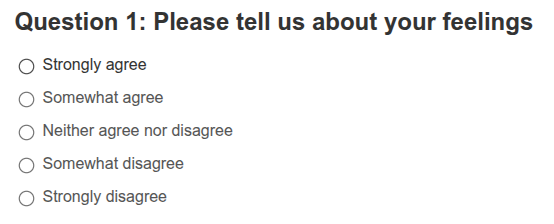
\includegraphics[scale=0.6]{./images/ls_en.png}
  \caption{Example of Likert Scale}
  \label{fig:ls}
\end{figure}

\begin{figure}[htbp]
  \centering
  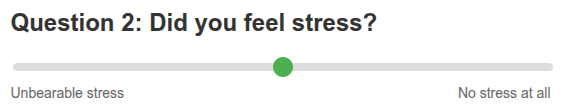
\includegraphics[scale=0.6]{./images/vas_en.png}
  \caption{Example of Visual Analog Scale}
  \label{fig:vas}
\end{figure}

\section{Experimental Procedure}
\subsection{Participants}
Twenty-four adults ($\geq 16$ years) with web service experience participated in this study. Participants were randomly assigned to two groups: character-by-character text output (Group A, $n = 12$) and full-text display (Group B, $n = 12$). The sample size was determined based on a power analysis for medium effect sizes (Cohen's $d = 0.8$) with $\alpha$ = 0.05 and power = 0.80.

All participants provided written informed consent after receiving detailed information about the study’s purpose, procedures, and data handling. The study protocol ensured that no personal information was collected beyond basic demographic data, and all data were used exclusively for academic purposes. Participants were informed of their right to withdraw from the study at any time without penalty.

The inclusion criteria required participants to have regular experience with web-based interfaces and normal or corrected-to-normal vision. The exclusion criteria included self-reported reading difficulties or visual impairments that might interfere with text processing. The between-subjects design eliminated concerns about practice effects or condition order influence.

\subsection{Materials and Apparatus}
The experimental questionnaire was developed using Unity, a cross-platform development environment provided by Unity Technologies, Inc.. This platform was selected for its capability to provide precise timing measurements and consistent, cross-platform performance. The application recorded the participant responses and timing data with millisecond precision.

The text stimulus consisted of an excerpt from Ryunosuke Akutagawa's short story ``The Nose,'' selected for its moderate complexity and cultural neutrality for the target population. The text length (approximately 200 characters) was chosen to provide sufficient reading material while maintaining a reasonable experimental session duration.

For the character-by-character condition, the text appeared at a fixed rate of one character per 0.1 seconds (equivalent to 600 characters per minute), based on Uetsuki and Horii's \cite{uetsuki2017} findings regarding optimal presentation rates. This rate was selected to be within the range of normal reading speeds while being slow enough to constrain faster reader speeds.

\subsection{Procedure}
The experimental session consisted of three sequential phases: orientation, text presentation, and evaluation phase. Each session lasted approximately 10-15 minutes and was conducted in a controlled environment with consistent lighting and minimal distractions.

\textbf{Phase 1: Orientation.} Participants first viewed an overview screen that explained the study’s purpose, procedure flow, and data handling policies. This phase ensured informed consent and familiarized the participants with the interface. Participants initiated the experiment by pressing a ``Start'' button, indicating their readiness to proceed.

\textbf{Phase 2: Text Presentation.} Upon entering the text section, the timing measurement began automatically. Group A participants initially observed blank screens with characters appearing sequentially at a predetermined rate. Participants in Group B saw the complete text immediately upon screen entry. Participants were instructed to read naturally and press a ``Next'' button upon completing their reading, which stopped the timing measurement and advanced to the evaluation phase.

\textbf{Phase 3: Evaluation.} Participants completed VAS ratings for all four dimensions (readability, stress, understanding, and memorability) using continuous sliders scaled from 0 to 1000 (later normalized to 0-100 for analysis). The evaluation interface presented each dimension on a separate screen to prevent response bias. The participants concluded by pressing an ``End'' button, completing the session.

\subsection{Statistical Analysis}
Data analysis employed appropriate parametric and non-parametric tests depending on the distributional assumptions. Levene's test was used to assess the variance homogeneity for each dependent variable. Independent samples t-tests were conducted for variables meeting parametric assumptions, whereas Welch's t-test was applied when variance homogeneity was violated.

Effect sizes were calculated using Cohen's d to assess practical significance beyond statistical significance. All analyses were conducted using appropriate statistical software with $\alpha$ = 0.05 as the significance criterion. Missing data procedures were established but were not needed as the study achieved a 100\% completion rate.

\section{Results}
\subsection{Descriptive Statistics}
The character-by-character text output Group A designated as Group A, and the full-text display group was designated as Group B. Table \ref{tab:data_a} presents the complete dataset for Group A participants, whereas Table \ref{tab:data_b} shows the corresponding data for Group B participants. Summary statistics, including minimum values, maximum values, means, medians, and standard deviations for both groups, are provided in Tables \ref{tab:statistics_a} and \ref{tab:statistics_b}.

A visual representation of the data distributions is provided through box plots and violin plots in Fig. \ref{fig:subjective} and Fig. \ref{fig:time}. These visualizations reveal notable patterns in the data, including the compressed variance in Group A’s reading times and the differential distributions across subjective rating dimensions.

\begin{table}[htbp]
  \centering
  \caption{Experimental Results for Group A}
  \label{tab:data_a}
  \begin{tabular}{rrrrr}
    \toprule
    Readability & Stress & Understanding & Memorability & Time[s]   \\
    \midrule
    19          & 46     & 38            & 53           & 106.849   \\
    24          & 56     & 50            & 68           & 75.3085   \\
    77          & 22     & 55            & 20           & 77.16992  \\
    29          & 48     & 45            & 20           & 78.85937  \\
    72          & 82     & 59            & 39           & 76.40662  \\
    16          & 91     & 36            & 9            & 76.52671  \\
    36          & 65     & 35            & 34           & 75.40749  \\
    64          & 65     & 72            & 80           & 96.43768  \\
    27          & 78     & 45            & 30           & 75.296991 \\
    18          & 66     & 0             & 19           & 79.46642  \\
    30          & 74     & 26            & 25           & 76.2334   \\
    13          & 90     & 22            & 19           & 76.52383  \\
    \bottomrule
  \end{tabular}
\end{table}

\begin{table}[htbp]
  \centering
  \caption{Experimental Results for Group B}
  \label{tab:data_b}
  \begin{tabular}{rrrrr}
    \toprule
    Readability & Stress & Understanding & Memorability & Time[s]  \\
    \midrule
    28          & 56     & 28            & 12           & 46.33347 \\
    33          & 42     & 27            & 23           & 109.1233 \\
    36          & 41     & 39            & 33           & 51.2507  \\
    31          & 66     & 12            & 42           & 48.1253  \\
    79          & 17     & 11            & 60           & 50.5961  \\
    50          & 0      & 25            & 50           & 24.9764  \\
    51          & 38     & 23            & 44           & 65.4829  \\
    36          & 29     & 31            & 31           & 52.6615  \\
    26          & 46     & 16            & 61           & 49.2248  \\
    67          & 55     & 59            & 28           & 69.1192  \\
    44          & 27     & 24            & 21           & 77.589   \\
    37          & 88     & 18            & 42           & 53.9858  \\
    \bottomrule
  \end{tabular}
\end{table}

\begin{table}[htbp]
  \centering
  \caption{Summary Statistics for Group A}
  \label{tab:statistics_a}
  \resizebox{\textwidth}{!}{%
  \begin{tabular}{lrrrrr}
    \toprule
            & Readability & Stress   & Understanding & Memorability & Time[s]  \\
    \midrule
    Minimum & 13          & 22       & 0             & 9            & 75.3     \\
    Median  & 28          & 65.5     & 41.5          & 27.5         & 76.53    \\
    Mean    & 35.42       & 65.25    & 40.25         & 34.67        & 80.87    \\
    Maximum & 77          & 91       & 72            & 80           & 106.85   \\
    Std Dev & 22.581      & 20.04597 & 18.88783      & 21.77711     & 10.03614 \\
    \bottomrule
  \end{tabular}%
  }
\end{table}

\begin{table}[htbp]
  \centering
  \caption{Summary Statistics for Group B}
  \label{tab:statistics_b}
  \resizebox{\textwidth}{!}{%
  \begin{tabular}{lrrrrr}
    \toprule
            & Readability & Stress   & Understanding & Memorability & Time[s]  \\
    \midrule
    Minimum & 26          & 0        & 11            & 12           & 24.98    \\
    Median  & 36.5        & 41.5     & 24.5          & 37.5         & 51.96    \\
    Mean    & 43.17       & 42.08    & 26.08         & 37.25        & 58.21    \\
    Maximum & 79          & 88       & 59            & 61           & 109.12   \\
    Std Dev & 16.17424    & 23.10631 & 13.09725      & 15.32155     & 20.72025 \\
    \bottomrule
  \end{tabular}%
  }
\end{table}

\begin{figure}[htbp]
  \centering
  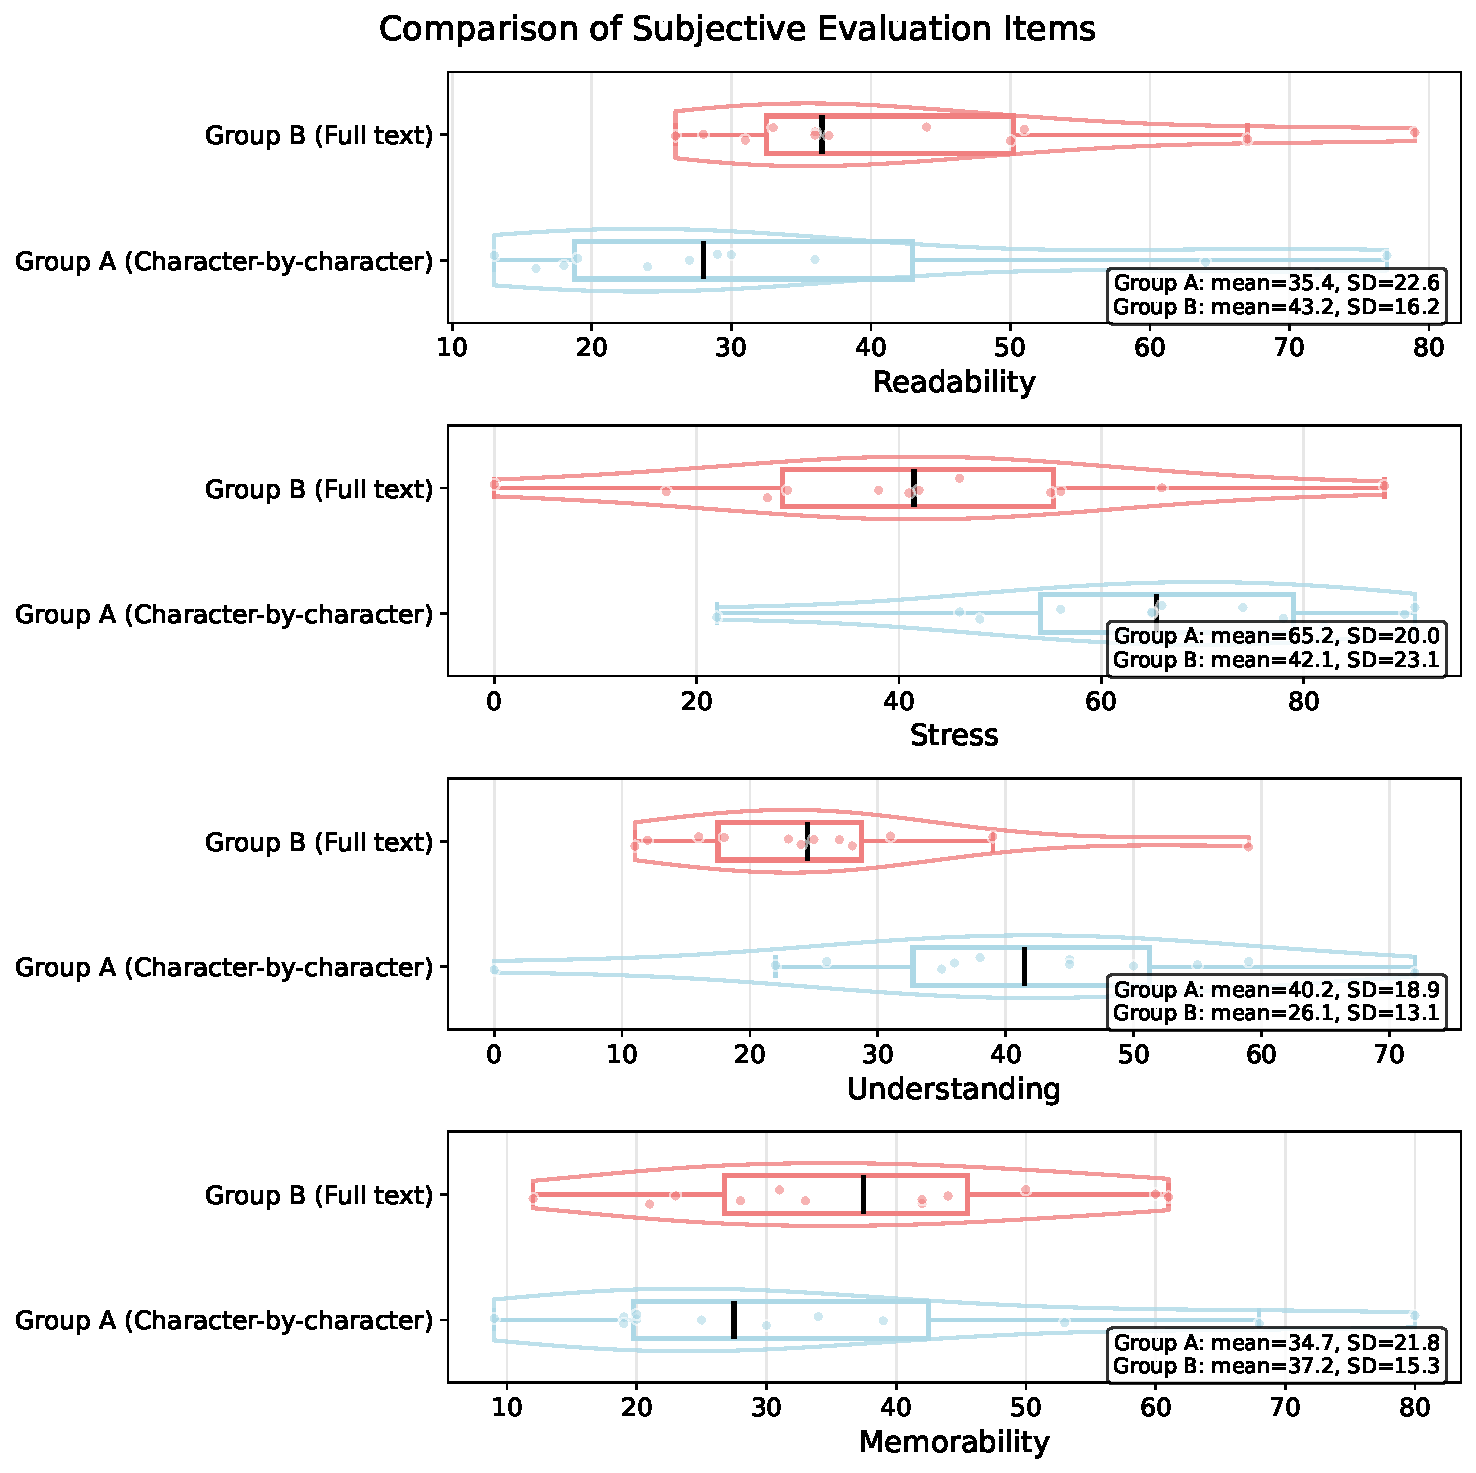
\includegraphics[width=\textwidth]{./images/subjective_en.pdf}
  \caption{Distribution of Each Item}
  \label{fig:subjective}
\end{figure}

\begin{figure}[htbp]
  \centering
  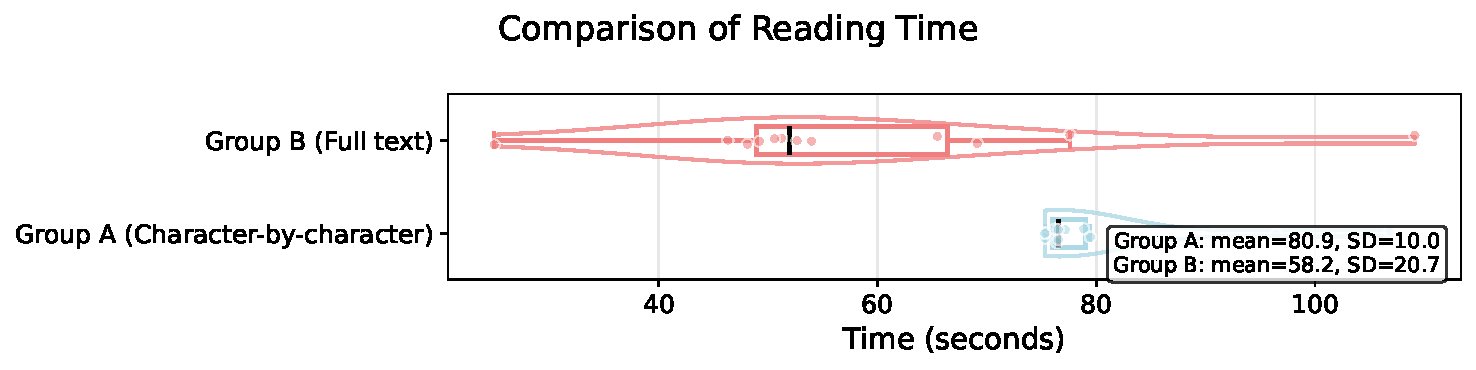
\includegraphics[width=\textwidth]{./images/time_en.pdf}
  \caption{Distribution of Reading Time}
  \label{fig:time}
\end{figure}

\subsection{Inferential Statistics}
To investigate the significant differences between Groups A and B across all measured dimensions, we conducted comprehensive statistical tests following established protocols. For each variable, mean-centered Levene's test was used to assess variance homogeneity to determine the appropriate t-test procedures. Independent samples t-tests were performed for variables meeting homogeneity assumptions, while Welch's t-test was applied when equal variances could not be assumed.

The complete analysis results are summarized in Table \ref{tab:test}, which presents the variance homogeneity test outcomes, t-test results, and effect sizes for all measured dimensions. Statistical significance was evaluated against $\alpha$ = 0.05, and effect sizes were calculated using Cohen's d to assess practical significance.

The results revealed significant group differences in three of the five measured variables. For stress, understanding, and reading time, the p-values fell below the 0.05 significance threshold, indicating reliable differences between the presentation methods. Conversely, readability and memorability showed non-significant differences, suggesting comparable performance across the groups on these dimensions.

\begin{table}[htbp]
  \centering
  \caption{Analysis Results by Item}
  \label{tab:test}
  \resizebox{\textwidth}{!}{%
  \begin{tabular}{lccrrrr}
    \toprule
    Item          & Variance Homogeneity & Test    & df & $t$   & $p$-value & Cohen's $d$ \\
    \midrule
    Readability   & Homogeneous          & Student & 22 & -0.97 & 0.3443    & -0.39 \\
    Stress        & Homogeneous          & Student & 22 & 2.62  & 0.0155    & 1.07  \\
    Understanding & Homogeneous          & Student & 22 & 2.14  & 0.0441    & 0.87  \\
    Memorability  & Homogeneous          & Student & 22 & -0.34 & 0.7400    & -0.14 \\
    Time          & Homogeneous          & Student & 22 & 3.41  & 0.0025    & 1.39  \\
    \bottomrule
  \end{tabular}%
  }
\end{table}

\subsection{Statistical Significance Summary}
The statistical analysis yielded clear patterns of significance across the measured dimensions. For readability and memorability, the p-values exceeded 0.05 ($p = 0.344$ and $p = 0.74$, respectively), indicating no statistically significant differences between the presentation methods. These results suggest that both character-by-character and full-text display achieve comparable levels of perceived readability and memory retention.

Conversely, the three dimensions showed significant differences at the $\alpha = 0.05$ level. Stress demonstrated significant group differences $(p = 0.016)$, with character-by-character presentation producing higher stress responses. Understanding also showed significant differences $(p = 0.044)$, with character-by-character presentations yielding higher understanding scores. Reading time revealed the strongest significant difference $(p = 0.003)$, with full-text display enabling faster task completion.

These statistical findings provide robust evidence for the differential effects of text-presentation methods on specific aspects of user experience while confirming comparable effects on others. The results suggest that the presentation method primarily affects the temporal and affective dimensions rather than fundamental readability or memory processes.

\section{Results and Discussion}
\subsection{Statistical Analysis Results}
Statistical analysis revealed significant differences between character-by-character text output (Group A) and full-text display (Group B) in three of the five measured variables. The results demonstrate a complex pattern of trade-offs between the two presentation methods’ effectiveness.

For the stress dimension, Group A participants reported significantly higher stress levels $(M = 65.25, SD = 20.05)$ than Group B participants $(M = 42.08, SD = 23.11), t(22) = 2.62, p = 0.016$. This finding aligns with Longo et al.'s \cite{longo2018} observations that mental workload directly impacts user experience. The elevated stress levels in character-by-character presentation may be attributed to the temporal constraints imposed by the fixed presentation rate, which conflicts with the individual reading preferences identified by Uetsuki and Horii \cite{uetsuki2017}.

Interestingly, the understanding dimension showed an opposite pattern, with Group A participants reporting significantly higher understanding scores $(M = 40.25, SD = 18.89)$ than Group B participants $(M = 26.08, SD = 13.10), t(22) = 2.14, p = 0.044$. This suggests that despite causing more stress, character-by-character presentation may facilitate deeper text processing, possibly due to the enforced pacing that prevents skimming behavior.

The time analysis revealed that Group B completed reading significantly faster $(M = 58.21s, SD = 20.72)$ than Group A $(M = 80.87s, SD = 10.03), t(22) = 3.41, p = 0.003$. The smaller variance in Group A's reading times indicates that the character-by-character presentation rate effectively controlled the minimum reading duration, supporting Primativo et al.'s \cite{primativo2016} findings about the relationship between presentation rate and reading speed limits.

\subsection{Interpretation of Non-Significant Results}
The absence of significant differences in the readability and memorability dimensions provides important insights. The readability scores showed no significant difference between the groups (Group A: $M = 35.42$, Group B: $M = 43.17, p = 0.344$), suggesting that both presentation methods achieved comparable perceived legibility. This finding is consistent with García-Pérez's \cite{garcia-perez2023} work on measurement precision, indicating that the VAS methodology successfully captured subtle differences in some dimensions while revealing genuine similarities in others.

Similarly, memorability scores showed no significant difference (Group A: $M = 34.67$, Group B: $M = 37.25, p = 0.74$), which may reflect the complex relationship between presentation method and retention identified by Amadieu and Salmerón \cite{amadieu2009}. The lack of difference could indicate that memory consolidation occurs independently of presentation timing within the tested duration.

\subsection{Theoretical Implications}
These findings contribute to the theoretical understanding of dynamic text presentation in multiple ways. First, they provide empirical evidence of the trade-off between cognitive load and comprehension depth in digital interfaces. The higher stress but improved understanding in character-by-character presentation suggests that controlled pacing may enhance text processing at the cost of user comfort.

Second, the results support Darejeh and Singh's \cite{darejeh2024} emphasis on multidimensional cognitive load assessment. The differential effects across the stress, understanding, and time dimensions highlight the importance of comprehensive evaluation frameworks rather than single-metric assessments.

Third, this study extends Kühlmann et al.'s \cite{kuhlmann2016} validation of VAS in digital contexts by demonstrating its sensitivity to subtle differences in text presentation methods. The ability to detect significant differences in three of the five dimensions while appropriately identifying non-significant effects in the others supports the validity of the methodology.

\section{Limitations and Future Directions}
\subsection{Sample and Methodology Limitations}
This study has several limitations that should be addressed in future research. The sample size of 24 participants, while sufficient for detecting the observed effect sizes, limited the generalizability of the findings. Future studies should employ larger and more diverse samples to enhance external validity and enable subgroup analyses based on reading proficiency or age groups.

The fixed character presentation rate (0.1 s per character) represents another limitation. Uetsuki and Horii \cite{uetsuki2017} demonstrated individual variations in optimal presentation rates, suggesting that personalized timing may yield different results. Future research should investigate adaptive presentation rates that adjust to individual reading speed.

The choice of literary text (Akutagawa's ``The Nose'') may have influenced the results due to its cultural specificity and literary complexity. Amadieu and Salmerón's \cite{amadieu2009} work on prior knowledge effects suggests that text familiarity could moderate the observed differences. Future studies should examine the effects across different text types, complexity levels, and subject domains.

\subsection{Methodological Considerations}
Exclusive reliance on subjective measures, while appropriate for assessing user experience, should be complemented by objective measures in future research. Eye-tracking data, physiological measures, and comprehension testing can provide converging evidence for the observed effects and reveal the underlying cognitive mechanisms.

Although the experimental setting was controlled, it may not have reflected natural reading contexts. Future research should investigate these effects in ecologically valid environments, such as actual web applications or mobile interfaces, to enhance their practical relevance.

\subsection{Directions for Future Research}
Several promising research directions have emerged from this study. First, investigating optimal presentation rates tailored to individual differences could resolve the stress-understanding trade-off observed here. Adaptive systems that adjust timing based on real-time user feedback represent a particularly promising avenue for research.

Second, examining the long-term effects of different presentation methods on learning and retention can inform educational technology design. The observed understanding advantage for character-by-character presentations warrants investigation in learning contexts.

Third, exploring the effects of presentation methods on different user populations (e.g., older adults and individuals with reading difficulties) could reveal important accessibility implications. The stress differences observed here may be particularly relevant for users with cognitive processing differences.

\section{Conclusion}
This study provides empirical evidence for the differential effects of character-by-character versus full-text display methods on user experience in web interfaces. The findings reveal a fundamental trade-off: character-by-character presentation enhances understanding but increases stress and reading time compared to full-text display.

The significant differences in stress $(p = 0.016)$, understanding $(p = 0.044)$, and time $(p = 0.003)$ dimensions, combined with non-significant effects on readability and memorability, suggest that these presentation methods affect different aspects of the reading experience through distinct cognitive pathways. The character-by-character method appears to enforce deeper processing at the cost of user autonomy and comfort level.

These findings have practical implications for the design of interfaces. For applications prioritizing comprehension and learning, character-by-character presentation may be beneficial, despite the increased cognitive load. Conversely, for information browsing and efficiency-focused tasks, full-text display appears more appropriate.

The optimal application of these findings requires consideration of context-specific factors, including user goals, content type, and task requirements. Future research should focus on developing adaptive presentation systems that can dynamically adjust display methods according to user preferences and task demands.

The limitations of this study, including the sample size and text selection, indicate areas for methodological improvement. Nevertheless, the robust statistical findings and theoretical grounding provide a solid foundation for evidence-based interface-design decisions. The successful application of the VAS methodology to interface evaluation also contributes to an expanding toolkit for usability assessment in digital environments.

This study demonstrates that text presentation methods significantly impact user experience in measurable ways. By continuing to investigate these effects through rigorous empirical methods, the field can develop a more nuanced understanding of how interface design choices affect human cognition and user satisfaction in digital environments.

\bibliography{refworks}

\end{document}
